% Options for packages loaded elsewhere
\PassOptionsToPackage{unicode}{hyperref}
\PassOptionsToPackage{hyphens}{url}
\PassOptionsToPackage{dvipsnames,svgnames,x11names}{xcolor}
%
\documentclass[
]{article}
\usepackage{amsmath,amssymb}
\usepackage{lmodern}
\usepackage{iftex}
\ifPDFTeX
  \usepackage[T1]{fontenc}
  \usepackage[utf8]{inputenc}
  \usepackage{textcomp} % provide euro and other symbols
\else % if luatex or xetex
  \usepackage{unicode-math}
  \defaultfontfeatures{Scale=MatchLowercase}
  \defaultfontfeatures[\rmfamily]{Ligatures=TeX,Scale=1}
\fi
% Use upquote if available, for straight quotes in verbatim environments
\IfFileExists{upquote.sty}{\usepackage{upquote}}{}
\IfFileExists{microtype.sty}{% use microtype if available
  \usepackage[]{microtype}
  \UseMicrotypeSet[protrusion]{basicmath} % disable protrusion for tt fonts
}{}
\makeatletter
\@ifundefined{KOMAClassName}{% if non-KOMA class
  \IfFileExists{parskip.sty}{%
    \usepackage{parskip}
  }{% else
    \setlength{\parindent}{0pt}
    \setlength{\parskip}{6pt plus 2pt minus 1pt}}
}{% if KOMA class
  \KOMAoptions{parskip=half}}
\makeatother
\usepackage{xcolor}
\usepackage[margin=1in]{geometry}
\usepackage{longtable,booktabs,array}
\usepackage{calc} % for calculating minipage widths
% Correct order of tables after \paragraph or \subparagraph
\usepackage{etoolbox}
\makeatletter
\patchcmd\longtable{\par}{\if@noskipsec\mbox{}\fi\par}{}{}
\makeatother
% Allow footnotes in longtable head/foot
\IfFileExists{footnotehyper.sty}{\usepackage{footnotehyper}}{\usepackage{footnote}}
\makesavenoteenv{longtable}
\usepackage{graphicx}
\makeatletter
\def\maxwidth{\ifdim\Gin@nat@width>\linewidth\linewidth\else\Gin@nat@width\fi}
\def\maxheight{\ifdim\Gin@nat@height>\textheight\textheight\else\Gin@nat@height\fi}
\makeatother
% Scale images if necessary, so that they will not overflow the page
% margins by default, and it is still possible to overwrite the defaults
% using explicit options in \includegraphics[width, height, ...]{}
\setkeys{Gin}{width=\maxwidth,height=\maxheight,keepaspectratio}
% Set default figure placement to htbp
\makeatletter
\def\fps@figure{htbp}
\makeatother
\setlength{\emergencystretch}{3em} % prevent overfull lines
\providecommand{\tightlist}{%
  \setlength{\itemsep}{0pt}\setlength{\parskip}{0pt}}
\setcounter{secnumdepth}{-\maxdimen} % remove section numbering
\usepackage{booktabs}
\usepackage{longtable}
\usepackage{array}
\usepackage{multirow}
\usepackage{wrapfig}
\usepackage{float}
\usepackage{colortbl}
\usepackage{pdflscape}
\usepackage{tabu}
\usepackage{threeparttable}
\usepackage{threeparttablex}
\usepackage[normalem]{ulem}
\usepackage{makecell}
\usepackage{xcolor}
\ifLuaTeX
  \usepackage{selnolig}  % disable illegal ligatures
\fi
\IfFileExists{bookmark.sty}{\usepackage{bookmark}}{\usepackage{hyperref}}
\IfFileExists{xurl.sty}{\usepackage{xurl}}{} % add URL line breaks if available
\urlstyle{same} % disable monospaced font for URLs
\hypersetup{
  pdftitle={Wycena oraz analiza opcji amerykańskich i europejskich w modelu dwumianowym},
  pdfauthor={Tomasz Kąkol, Jan Kozłowski, Aleksander Walis},
  colorlinks=true,
  linkcolor={Maroon},
  filecolor={Maroon},
  citecolor={Blue},
  urlcolor={blue},
  pdfcreator={LaTeX via pandoc}}

\title{Wycena oraz analiza opcji amerykańskich i europejskich w modelu
dwumianowym}
\usepackage{etoolbox}
\makeatletter
\providecommand{\subtitle}[1]{% add subtitle to \maketitle
  \apptocmd{\@title}{\par {\large #1 \par}}{}{}
}
\makeatother
\subtitle{Wstęp do Inżynierii Finansowej - Projekt}
\author{Tomasz Kąkol, Jan Kozłowski, Aleksander Walis}
\date{}

\begin{document}
\maketitle

\renewcommand*\contentsname{Spis treści}
{
\hypersetup{linkcolor=}
\setcounter{tocdepth}{2}
\tableofcontents
}
\newpage

\hypertarget{wprowadzenie}{%
\section{Wprowadzenie}\label{wprowadzenie}}

Głównym celem raportu jest analiza modelu dwumianowego wyceny opcji
waniliowych typu put i call na aktywa nie wypłacające dywidend.
Rozpoczniemy od przedstawienia ogólnych założeń dotyczących modelu wraz
z jego przykładowym zastosowaniem przy pewnych ustalonych parametrach.
Następnie, zajmiemy się zbadaniem wrażliwości wyceny wynikającej z
modelu ze względu na zmianę parametrów modelu oraz porównamy różnicę w
wynikach między opcjami europejskimi i amerykańskimi. Przyjrzymy się
również składowi portfela zabezpieczającego wyceniane opcje oraz jego
zmianom przy rozwoju ceny aktywa bazowego.

\hypertarget{zaux142oux17cenia-dotyczux105ce-modelu}{%
\section{Założenia dotyczące
modelu}\label{zaux142oux17cenia-dotyczux105ce-modelu}}

Zakładamy dwumianowy model rynku, w którym aktywo bazowe (nie
wypłacające dywidend) warte w chwili \(t\) kwotę \(S_t\) może w kolejnym
kroku (tj. po upływie pewnej ustalonej ilości czasu, oznaczanej przez
\(\Delta t\)) być warte \(S_t \cdot u\) lub \(S_t \cdot d\), gdzie
\(u = e^{\sigma \sqrt{\Delta t}}\) i \(d = e^{-\sigma \sqrt{\Delta t}}\)
są współczynnikami odpowiednio wzrostu i spadku ceny, kontrolowanymi
przez parametr zmienności \(\sigma\). Poza aktywem bazowym dysponujemy
równiez możliwością inwestycji lub pożyczki ze stałą stopą wolną od
ryzyka \(r\) (w każdym okresie, zakładamy oprocentowanie ciągłe).

Przy takich założeniach wyznaczamy wartość opcji (o zapadalności \(T\)
lat i cenie wykonania \(K\)) na chwilę zero. Rozpoczynamy od wyznaczenia
możliwych wartości opcji w chwili \(T\), czyli po prostu wartości
wewnetrznych (dla opcji typu call \(\max (S_T - K, 0)\), a dla opcji
typu put \(\max (K - S_T, 0)\)); następnie, cofając się o kolejne kroki
w czasie wyznaczamy wartość opcji w oparciu o metodę \(\Delta\)-hedgingu
(lub równoważnie, korzystając z założenia o mierze obojętnej na ryzyko,
tj. wartość opcji jest zdyskontowaną wartością oczekiwaną jej przyszłego
\emph{payoffu}), przy czym, w przypadku opcji amerykańskich porównujemy
uzyskaną wartość z wartością wewnętrzną opcji i bierzemy większą z nich
(ze względu na możliwość wcześniejszego wykonania opcji). Kontynuując
ten proces, finalnie otrzymujemy wartość opcji w chwili początkowej.

\hypertarget{przykux142adowe-zastosowania-modelu}{%
\section{Przykładowe zastosowania
modelu}\label{przykux142adowe-zastosowania-modelu}}

W tym rozdziale przedstawimy przykładowe zastosowanie modelu do wyceny
opcji. Jak już wspomnieliśmy, będziemy rozważać następujące cztery
przypadki:

\begin{itemize}
\item
  opcje europejskie typu call i put,
\item
  opcje amerykańskie typu call i put.
\end{itemize}

Przyjmujemy następujące parametry, na podstawie których dokonamy
przykładowej wyceny: \[
S_o = 50,\;\; K = 48,\;\; T = 2,\;\; \Delta t = 1/12,\;\; \sigma = 0.3,\;\; r = 0.02
\] W następnych dwóch podrozdziałach zaprezentujemy uzyskane wyniki dla
każdego z przypadków, porównamy je między sobą i wyciągniemy wnioski.
Zanim jednak do tego przejdziemy, krótko opiszemy strukturę uzyskanego
modelu dla takich parametrów. Zauważmy, że ze względu na przyjęte
wartości parametrów \(T\) oraz \(\Delta t\) model zawiera aż \(325\)
wierzchołków (tj. rozważanych momentów w czasie z różną ceną aktywa
bazowego) z czego 25 z nich dotyczy chwili wygaśnięcia opcji. Wynika z
tego, że dokonujemy wyceny w oparciu o \(25\) możliwych przyszłych
wartości aktywa bazowego w owej chwili wygaśnięcia. Dla takiej liczby
wierzchołków wraz z przyjętą wysokością parametru zmienności \(\sigma\)
największą osiągalną wartością aktywa bazowego jest \(399.61\), co daje
przyrost rzędu \((399.61 - 50)/50 \approx 6.99\) (czyli o prawie
\(700 \%\)), a najmniejszą jest \(6.26\), co daje spadek rzędu
\((6.26 - 50)/50 \approx - 0.87\) (czyli o blisko \(87\%\)).

\hypertarget{wycena-opcji-europejskich-call-i-put}{%
\subsection{Wycena opcji europejskich call i
put}\label{wycena-opcji-europejskich-call-i-put}}

Rozpoczniemy od przykładowej wyceny opcji europejskich. Po dokonaniu
wyceny omawianym modelem dla ustalonych parametrów, wartość opcji w
chwili zero wynosi (w zaokrągleniu do dwóch miejsc po przecinku):

\begin{itemize}
\item
  w przypadku opcji call: \(10.19\),
\item
  w przypadku opcji put: \(6.31\).
\end{itemize}

Jak widzimy, wartość opcji call jest istotnie wyższa od wartości opcji
put dla tych parametrów. Nie jest to zaskoczeniem, bowiem zgadza się z
parytetem put-call - zauważmy, że przy przyjętych parametrach zachodzi
relacja \(S_0 \ge K > 0\), a z parytetu put-call mamy: \[
C_0 - P_0 = S_0 - Ke^{-rT} \ge K - Ke^{-rT} = K(1 - e^{-rT}) > 0
\] gdzie \(C_0\) i \(P_0\) są cenami odpowiednio opcji call i put w
chwili zero (zakładamy też, że \(r > 0\)). Analogicznymi
przekształceniami możemy uzyskać wartość parametru \(K\) tak, aby (przy
pozostałych parametrach niezmienionych) relacja uzyskanych wartości
opcji call i put się odwróciła.

\hypertarget{wycena-opcji-amerykaux144skich-call-i-put}{%
\subsection{Wycena opcji amerykańskich call i
put}\label{wycena-opcji-amerykaux144skich-call-i-put}}

Przejdziemy teraz do przykładowej wyceny opcji amerykańskich.
Przypomnijmy na początku, że różnicą między tym rodzajem opcji, a
opcjami rodzaju europejskiego jest możliwość wykonania opcji w dowolnym
momencie - ma to oczywiście znaczący wpływ na jej wartość. Po dokonaniu
wyceny omawianym modelem dla ustalonych parametrów, wartość opcji w
chwili zero wynosi (w zaokrągleniu do dwóch miejsc po przecinku):

\begin{itemize}
\item
  w przypadku opcji call: \(10.19\),
\item
  w przypadku opcji put: \(6.47\).
\end{itemize}

Jak widzimy, relacja między uzyskanymi wartościami jest taka sama jak w
przypadku opcji europejskich. Tym razem jednak, nie jesteśmy w stanie
powiedzieć że jest to rezultat zgodny z parytetem put-call, bowiem nie
obowiązuje on w przypadku opcji amerykańskich. Ze względu na możliwość
wcześniejszego wykonania opcji relacja między cenami opcjami obu typów
jest znacznie bardziej skomplikowana.

\hypertarget{poruxf3wnanie-rozwaux17canych-opcji-amerykaux144skich-i-europejskich}{%
\subsection{Porównanie rozważanych opcji amerykańskich i
europejskich}\label{poruxf3wnanie-rozwaux17canych-opcji-amerykaux144skich-i-europejskich}}

Zwróćmy jednak uwagę na pewną ciekawą prawidłowość - wartość opcji
europejskiej typu call jest równa wartości opcji amerykańskiej typu
call. Początkowo może się wydawać, że jest to zwykły przypadek
wynikający z akurat takiej konfiguracji parametrów; zauważmy jednak, że
jedynym czynnikiem mogącym wywołać zmianę w wycenie obu tych opcji jest
możliwość przedwczesnego wykonania opcji amerykańskiej. Jednakże, po
zbadaniu potencjalnej opłacalności takiego działania dochodzimy do
wniosku, że przedwczesne wykonanie opcji (przypomnijmy, zakładamy brak
wypłacanych dywidend dla aktywa bazowego) call nigdy nie jest opłacalne,
co poprawnie odzwierciedla wykorzystany przez nas model wyceny. Rozważmy
bowiem następujący scenariusz:\footnote{argumentacja zainspirowana
  rozdziałem 11.5 książki \emph{Options, futures and other derivatives}
  autorstwa Johna C. Hulla.} załóżmy, że w danej chwili przed upływem
ważności opcji aktywo bazowe warte jest 50 PLN, a cena wykonania wynosi
40 PLN. Jeśli zależy nam na posiadaniu owego aktywa, lepiej zapłacić
cenę wykonania później, ponieważ: (1) 40 PLN, które zapłacimy w
przyszłości warte jest mniej niż te, które zapłacilibyśmy teraz oraz (2)
istnieje szansa, że cena aktywa spadnie nawet poniżej ceny wykonania.
Jeśli natomiast nie interesuje nas posiadanie aktywa, a jedynie zarobek,
to bardziej opłacalnym działaniem jest sprzedanie całej opcji (której
cena musi być większa niż wartość wewnętrzna, tj. przychód z
natychmiastowego wykonania), lub sprzedanie krótko aktywa bazowego i
dostarczenie go w momencie wykonania opcji, kiedy to cena aktywa może
spaść nawet poniżej ceny wykonania.

Równości cen opcji europejskich i amerykańskich typu put oczywiście nie
zachodzi. W tym przypadku możliwość przedwczesnego wykonania opcji w
wielu momentach jest jak najbardziej działaniem optymalnym, a
argumentacja analogiczna do tej z powyższego akapitu oczywiście nie
znajduje zastosowania. Bierze się to między innymi z faktu, że spadek
(oraz jego tempo) ceny aktywa bazowego jest znacznie mniejszy (oraz
ograniczony!) od jego wzrostu w rozważanym przez nas modelu.

Przyjrzyjmy się teraz optymalnym momentom wykonania opcji put oraz
różnicy między wartościami amerykańskich i europejskich opcji put dla
rozważanych parametrów. Obie rzeczy przedstawiają poniższe ilustracje.

\begin{center}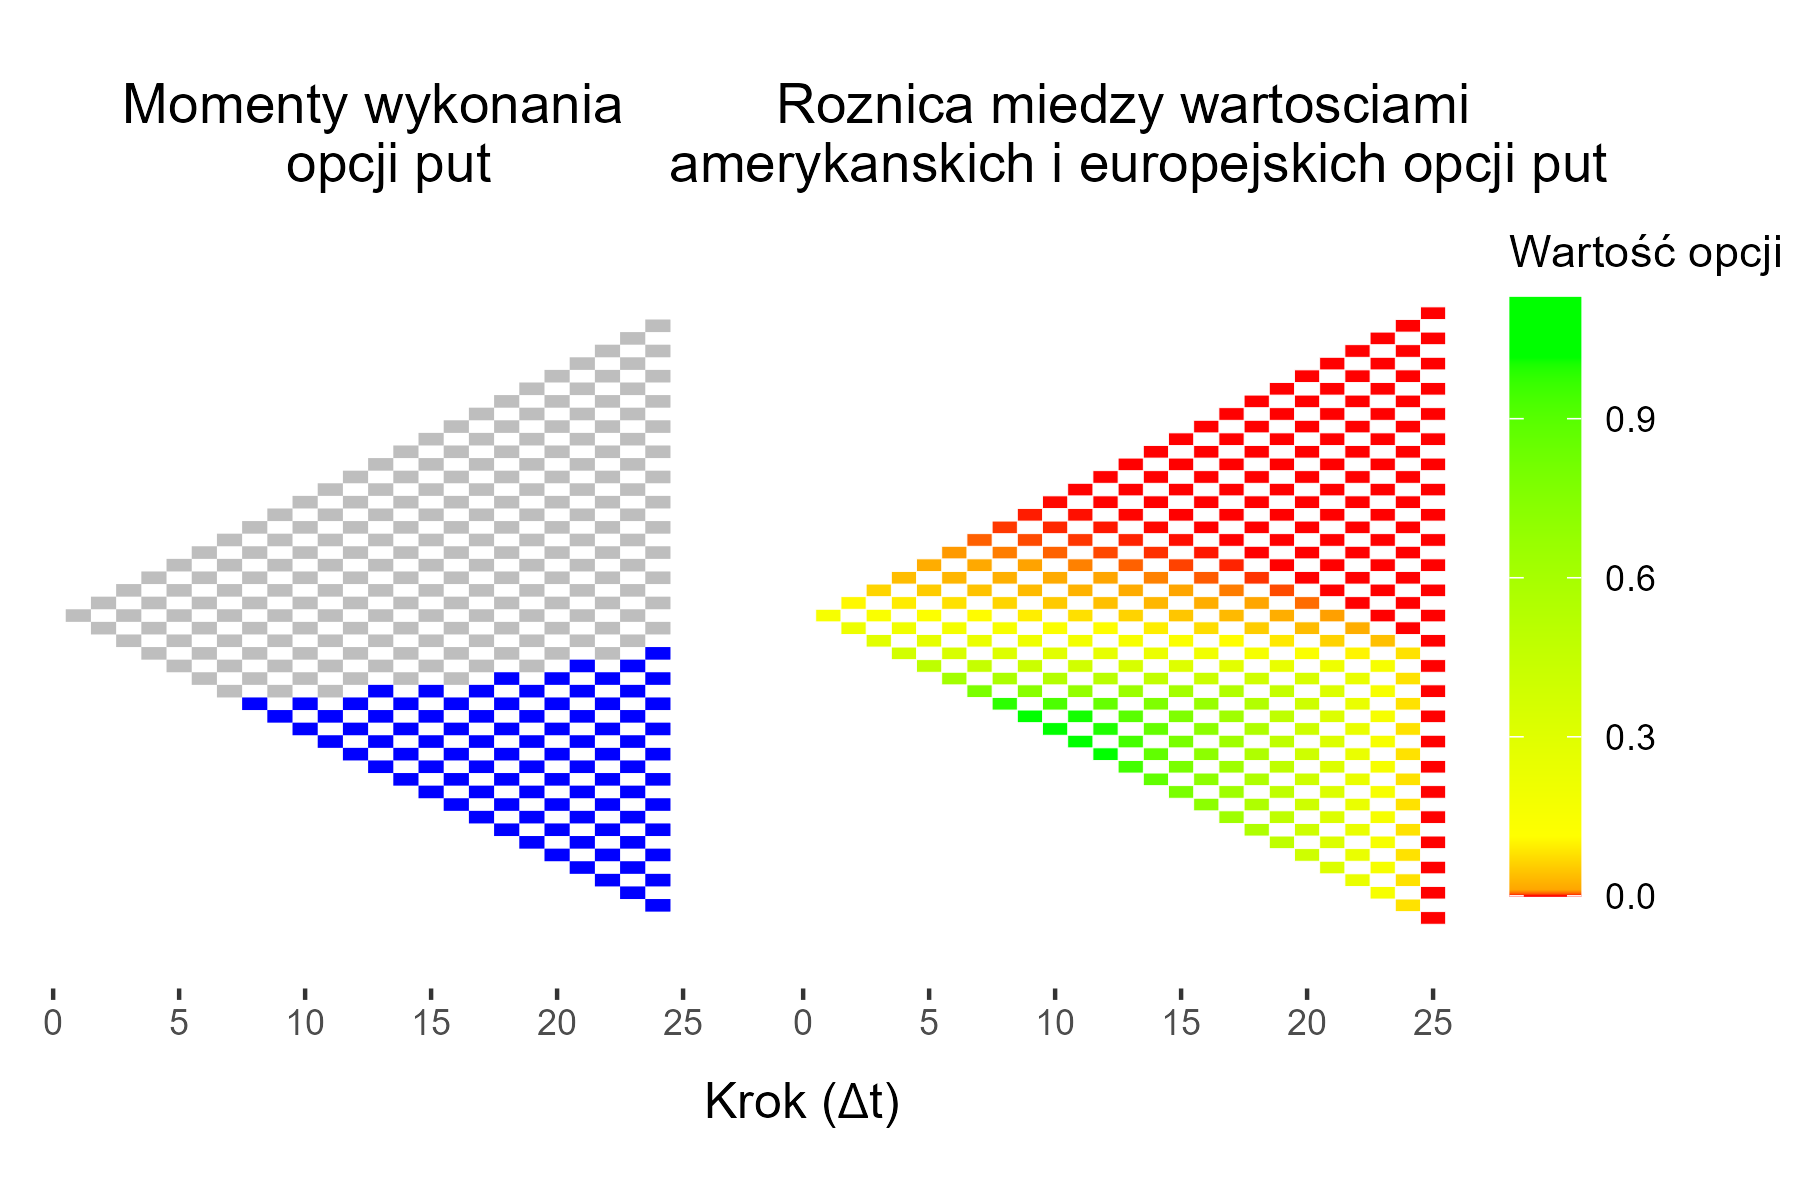
\includegraphics[width=0.75\linewidth,trim=0 10 0 10,clip]{wykresy/wykres} \end{center}

\emph{Rysunek 1. Drzewa wyceny opcji amerykańskich typu put. Rysunek po
lewej zawiera drzewo z momentami optymalnego wykonania opcji, gdzie
kolor niebieski odpowiada wierzchołkowi, który odpowiada momentowi w
czasie, kiedy wykonanie opcji jest optymalnym działaniem; w przeciwnym
wypadku wierzchołek oznaczony jest kolorem szarym. Rysunek po prawej
zawiera drzewo wyceny z różnicami wartości opcji w danym wierzchołku
między amerykańską i europejską opcją put.}

Rozpocznijmy od analizy momentów optymalnego wykonania. Jak widzimy na
drzewie wyceny, wykonanie opcji staje się optymalnym wyborem w dolnej
części drzewa, kiedy cena aktywa bazowego osiąga pewną niską wartość
(konkretnie \(27.27\)). Dla każdego następnego wierzchołka, w którym
cena aktywa jest owej niskiej wartości równa bądź mniejsza wykonanie
również jest opcją optymalną. Co do różnic cen między opcją amerykańską
a europejską, dokonajmy na początku pewnej trywialnej obserwacji -
wartość opcji amerykańskiej jest w każdym wierzchołku wyższa lub równa
od wartości opcji europejskiej (wynika to oczywiście z możliwości
przedwczesnego wykoniania). Największą różnicę w wartościach widzimy dla
wierzchołków znajdujących się nisko i w połowie drzewa, tj. dla tych,
dla których cena aktywa bazowego jest już dosyć niska, po upływie około
połowy czasu do wygaśnięcia opcji. Brak różnicy widzimy natomiast w
każdym z ostatnich wierzchołków (gdzie wartości są równe z oczywistych
względów) oraz w górnej części drzewa wyceny.

\hypertarget{analiza-wraux17cliwoux15bci-modelu}{%
\section{Analiza wrażliwości
modelu}\label{analiza-wraux17cliwoux15bci-modelu}}

W tym rozdziale zajmiemy się analizą wrażliwości wyceny modelu
dwumianowego. Jest to jedna z najważniejszych kwestii efektywności
modeli wyceny aktywów finansowych, bowiem ich parametryzacja często
opiera się na realizacjach pewnych zjawisk, które nie są znane osobom
wyceniającym dane aktywa. Prawdopodobnie najbardziej istotnym z tych
zjawisk jest zmienność rynku - w naszym przypadku jest to \emph{de
facto} pytanie o dobór wartości parametrów dotyczących zmienności ceny
aktywa bazowego, czyli parametr \(\sigma\) oraz wysokości stopy
procentowej \(r\). Problem odpowiedniej parametryzacji nie kończy się
jednak wyłącznie na dokładnej estymacji wartości dotyczących zmienność
rynku; równie ważna jest strona parametryzacji technicznej, tj. tej
dotyczącej wyłącznie struktury modelu, nie odnoszącej się bezpośrednio
do faktycznej rzeczywistości związanej z modelowanymi instrumentami
finansowymi - w naszym przypadku jest to przede wszystkim parametr
\(\Delta t\) kontrolujący liczbę `kroków' w modelu, którego zmiana może
mieć znaczący wpływ na finalną wycenę danej opcji.

W następnych dwóch podrozdziałach przeanalizujemy wpływ zmiany
pojedynczego parametru na zmianę wyceny opcji - rozpoczniemy od zbadania
zmian parametrów \(S_0, K, T, \sigma\) i \(r\), tj. tych bezpośrednio
odnoszących się do ogólnie pojętej sytuacji rynkowej, po czym przyjrzymy
się jakie zmiany wywołuje wykorzystanie innych wartości parametru
\(\Delta t\). W ostatnim, trzecim podrozdziale zbadamy wspólny wpływ
zmian w różnych parach parametrów.

\hypertarget{wpux142yw-zmiany-parametruxf3w-s_0-k-sigma-i-r}{%
\subsection{\texorpdfstring{Wpływ zmiany parametrów \(S_0, K, \sigma\) i
\(r\)}{Wpływ zmiany parametrów S\_0, K, \textbackslash sigma i r}}\label{wpux142yw-zmiany-parametruxf3w-s_0-k-sigma-i-r}}

Analizę wrażliwości wyceny na zmiany pojedynczych parametrów
rozpoczniemy od zbadania wpływu parametru \(S_0\) i \(K\), czyli
początkowej wartości aktywa bazowego i ceny wykonania opcji odpowiednio.
Za zakres zmienności obu parametru przyjmujemy przedział \([30, 80]\) (w
przykładowej wycenie przyjmowaliśmy \(S_0 = 50\) i \(K = 48\)).
Pozostałe parametry pozostają niezmienione, równe wcześniej
zaprezentowanym wartościom. Na poniższych wykresach przedstawiamy
uzyskane wyceny opcji call i put na chwilę zero (podzielone ze względu
na rodzaj opcji: a - amerykański, e - europejski), w zależności od
wartości wspomnianych parametrów.

\begin{center}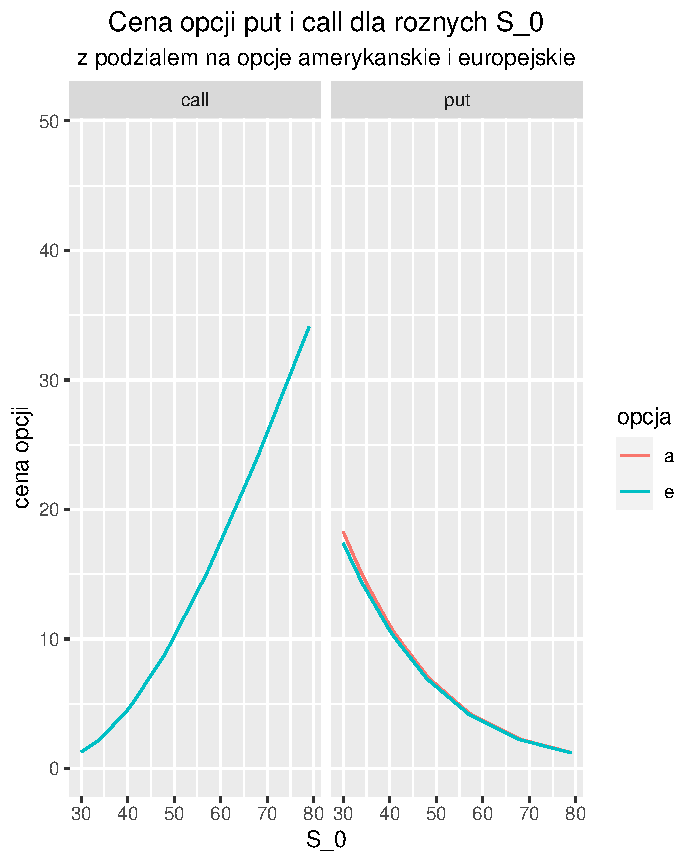
\includegraphics[width=0.4\linewidth]{wykresy/d_r_S0} 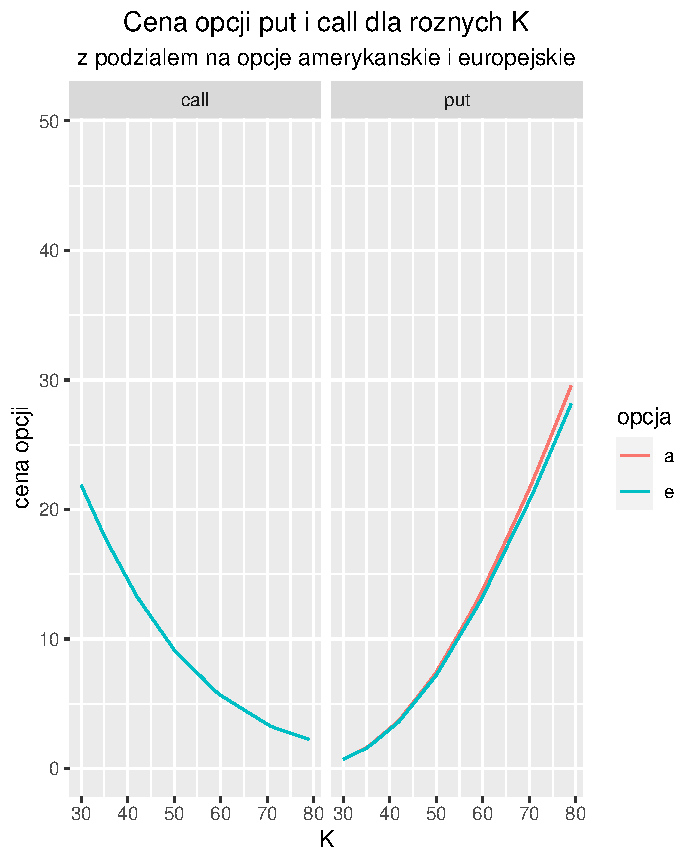
\includegraphics[width=0.4\linewidth]{wykresy/d_r_K} \end{center}

\emph{Rysunek 2. Wykres wartości opcji call i put w chwili zero w
zależności od wartości parametrów \(S_0\) i \(K\).}

Zanim rozpoczniemy dokładną analizę uzyskanych wyników zwróćmy uwagę na
fakt (który widoczny będzie również w następnych przypadkach), że wycena
opcji call dla opcji amerykańskich i europejskich jest równa - zjawisko
te opisaliśmy w poprzednim rozdziale. Wracając do badania wpływu
parametrów, zacznijmy od parametru \(S_0\). Jak widzimy na powyższym
wykresie, jego wzrost ma wyraźnie silny wpływ na wzrost wartości opcji
call i spadek wartości opcji put. W przypadku opcji call owy wzrost jest
zdaje się być bardzo szybki, natomiast spadek dla opcji call zdaje się
powoli stabilizować już przy \(S_0\) równym \(80\). Zauważmy jeszcze, że
różnice między wycenami opcji put rodzaju amerykańskiego i europejskiego
są minimalne.

Przejdźmy teraz do wpływu parametru \(K\). W tym przypadku również
widzimy silną zależność między jego wartością a uzyskaną wyceną - jednak
tym razem, wzrost parametru ma znaczący wpływ na spadek wartości opcji
call i wzrost wartości opcji put; również tutaj spadek zdaje się
stabilizować już przy \(K\) równym \(80\). Analogicznie jak w przypadku
parametru \(S_0\), różnice między wycenami opcji put rodzaju
amerykańskiego i europejskiego są niewielkie.

Następnymi parametrami, których wpływ na wycenę zbadamy, są \(\sigma\) i
\(r\), czyli czyli tzw. zmienność ceny aktywa bazowego (kontrolująca to
jak bardzo owa cena rośnie/maleje między sąsiadującymi wierzchołkami) i
stopa procentowa bez ryzyka odpowiednio. Za zakres zmienności parametru
\(\sigma\) przyjmujemy przedział \([0.05, 0.3]\) (w przykładowej wycenie
przyjmowaliśmy \(\sigma = 0.3\)), a dla parametru \(r\) przedział
\([-0.03, 0.2]\). Pozostałe parametry pozostają niezmienione, równe
wcześniej zaprezentowanym wartościom. Na poniższych wykresach
przedstawiamy uzyskane wyceny opcji call i put na chwilę zero
(podzielone ze względu na rodzaj opcji: a - amerykański, e -
europejski), w zależności od wartości wspomnianych parametrów.

\begin{center}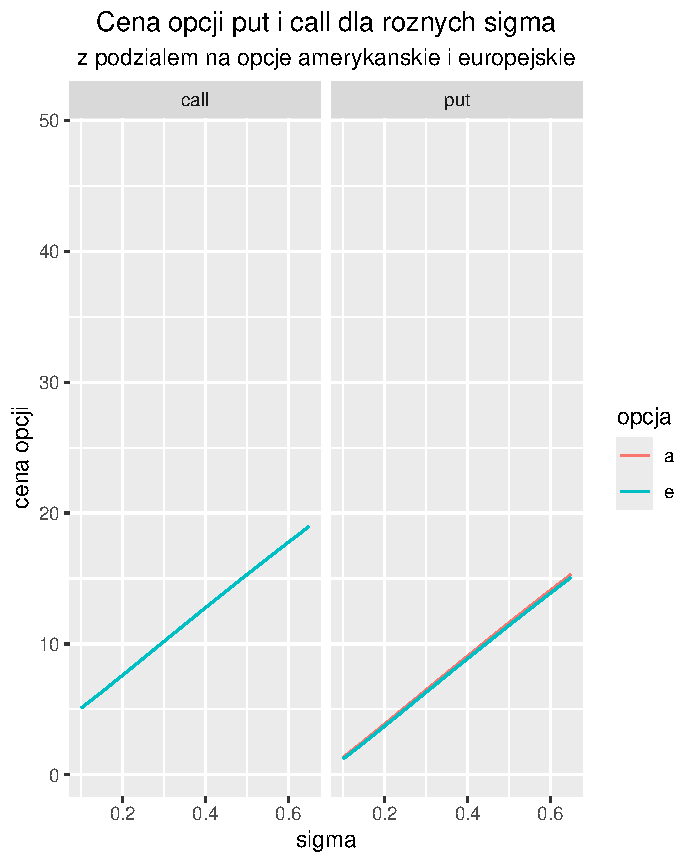
\includegraphics[width=0.4\linewidth]{wykresy/d_r_s} 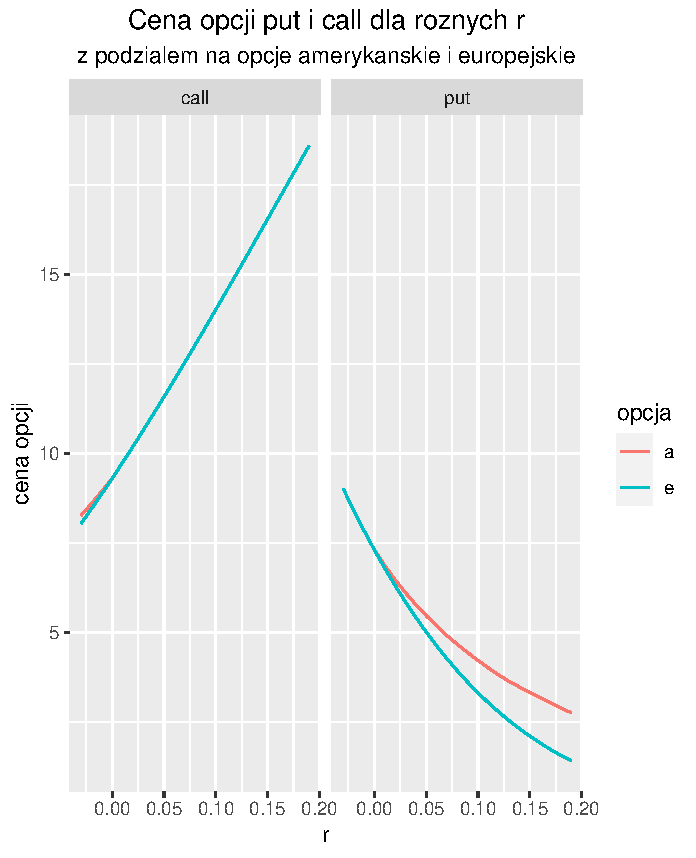
\includegraphics[width=0.4\linewidth]{wykresy/d_r_r} \end{center}

\emph{Rysunek 3. Wykres wartości opcji call i put w chwili zero w
zależności od wartości parametrów \(\sigma\) i \(r\).}

Zacznijmy od badania wpływu parametru \(\sigma\). Jak widzimy na
powyższych wykresach, jego wzrost ma pozytywny wpływ na wzrost wartości
zarówno opcji call jak i put. Porównując jednak poziom tego przyrostu z
tym uzyskanym dla poprzednich dwóch przypadków (tj. dla parametrów
\(S_0\) i \(K\)) widzimy, że jest on znacznie mniejszy, wynoszący
jedynie PLN; zauważmy również, że poziom tego przyrostu zdaje się być
równy dla obu typów opcji. Co do różnic między wartościami opcji put
rodzaju amerykańskiego i europejskiego, ponownie owe różnice są
minimalne.

Przejdźmy teraz do wpływu parametru \(r\). Jak widzimy na wykresach,
mamy do czynienia z tą samą zależnością jak w przypadku parametru
\(S_0\), tj. wraz ze wzrostem parametru \(r\) obserwujemy wzrost
wartości opcji call oraz spadek wartości opcji put. Zwróćmy jednak
szczególną uwagę na zakres dopuszczalnych wartości parametru -
dopuszczamy również ujemne wartości stopy procentowej bez ryzyka. Jest
to oczywiście wartość odpowiadająca dość niepowszechnym sytuacjom
rynkowym. Zauważmy, że w tym przypadku ceny opcji call rodzaju
europejskiego i amerykańskiego różnią się, na podstawie czego możemy
wywnioskować, że istnieją momenty optymalnego przedterminowego wykonania
opcji. Co do poziomu wzrostu jak i spadku wartości opcji obu typów,
warto odnotować że nie jest on zbyt duży - szczególnie, jeśli skupimy
się na najczęściej występujących wartościach stopy procentowej, tj.
takim w przedziale \([0.01, 0.1]\), wtedy ów poziom jest niewielki,
wynoszący \(\pm 1\) PLN.

\hypertarget{wpux142yw-zmiany-parametruxf3w-t-i-delta-t}{%
\subsection{\texorpdfstring{Wpływ zmiany parametrów \(T\) i
\(\Delta t\)}{Wpływ zmiany parametrów T i \textbackslash Delta t}}\label{wpux142yw-zmiany-parametruxf3w-t-i-delta-t}}

Ostatnimi parametrami, których wpływ na wycenę zbadamy, jest
\(\Delta t\) i \(T\), czyli czas mijający w trakcie jednego kroku w
drzewie wyceny oraz czas do wygaśnięcia opcji (podawany w latach)
odpowiednio. Oba parametry dotyczą czasu w rozważanym modelu, przy czym
wartość parametru \(\Delta t\) ma wpływ nie tylko na uzyskaną wartość
opcji, ale również na czas wykonania algorytmu dokonującego wyceny,
bowiem bezpośrednio determinuje on liczbę wierzchołków w drzewie. W
związku z tym, przeanalizujemy nie tylko uzyskane wartości opcji w
zależności od wartości tych parametrów, ale również wpływ wartości
parametru \(\Delta t\) na czas dokonania tej wyceny. Za zakres
zmienności parametru \(T\) przyjmujemy przedział \((0, 100]\) (w
przykładowej wycenie przyjmowaliśmy \(T = 2\)), a dla parametru
\(\Delta t\) przedział \((0, 0.5]\) (w przykładowej wycenie
przyjmowaliśmy \(\Delta t = 1/12\)). Pozostałe parametry pozostają
niezmienione, równe wcześniej zaprezentowanym wartościom. Rozpoczniemy
od analizy różnic w wycenie opcji - na poniższych wykresach
przedstawiamy uzyskane wyceny opcji call i put na chwilę zero
(podzielone ze względu na rodzaj opcji: a - amerykański, e -
europejski), w zależności od wartości wspomnianych parametrów.

\begin{center}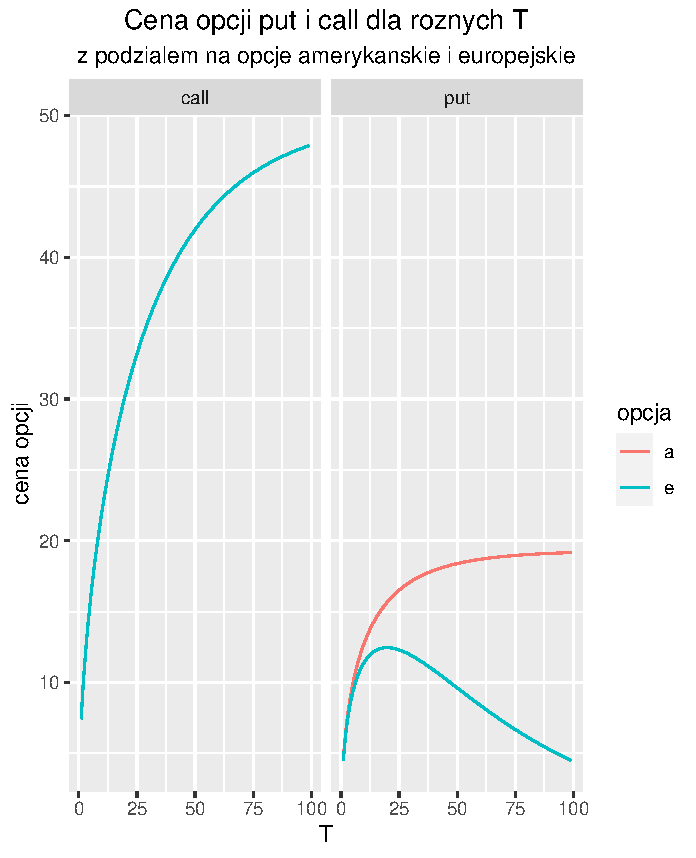
\includegraphics[width=0.4\linewidth]{wykresy/d_r_T} 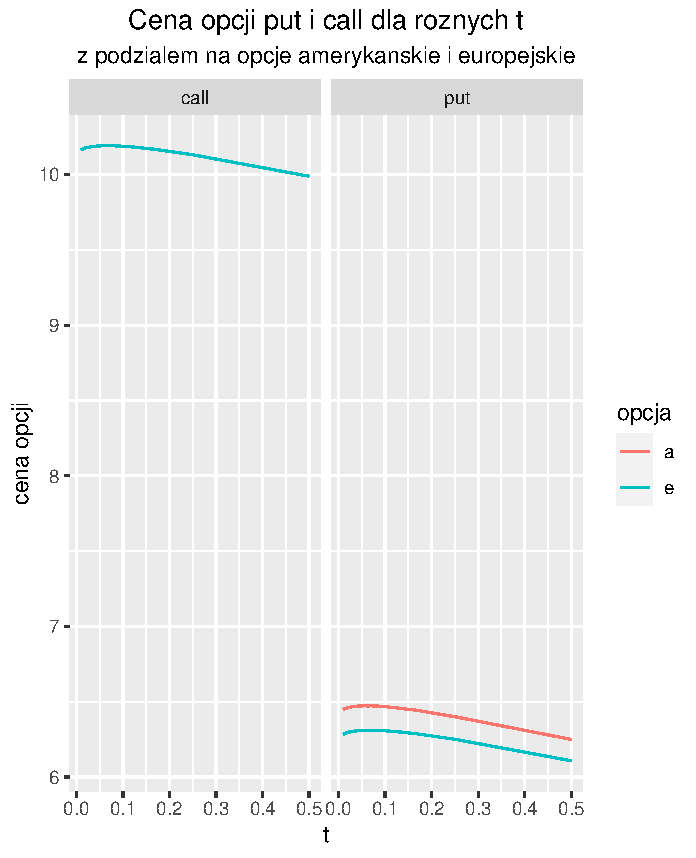
\includegraphics[width=0.4\linewidth]{wykresy/d_r_ot} \end{center}

\emph{Rysunek 4. Wykres wartości opcji call i put w chwili zero w
zależności od wartości parametrów \(T\) i \(\Delta t\).}

Rozpoczniemy od zbadania wpływu parametru \(T\). Dla opcji call jak i
dla opcji put typu amerykańskiego obserwujemy wzrost wartości opcji przy
wzroście parametru \(T\). W obu przypadkach zauważamy stabilizację
uzyskanej wyceny dla parametru \(T\) bliskiego \(100\), przy czym wzrost
wartości opcji call jest znacznie wyższy od wzrostu opcji put rodzaju
amerykańskiego. Zwróćmy równiez uwagę na znaczną różnicę w wartościach
między opcjami put rodzaju amerykańskiego i europejskiego - tak duża
różnica nie występowała w przypadku zmian innych parametrów.
Interesująca jest również dokładna zmienność wartość wyceny opcji
europejskiej typu put - początkowo wzrasta wraz ze wzrostem parametru
\(T\), a następnie maleje; zauważmy jednak, że rozważamy naprawdę duże
wartości parametru \(T\), raczej nie spotykane w praktyce. Jednak
ppodobnie niecodzienny kształt możemy uzyskać dla mniejszych \(T\), gdy
zwiększymy ``chaotyczność'' rynku, tzn. zmieniając parametry na
\(\sigma = 0.6,r = 0.3\)

\begin{center}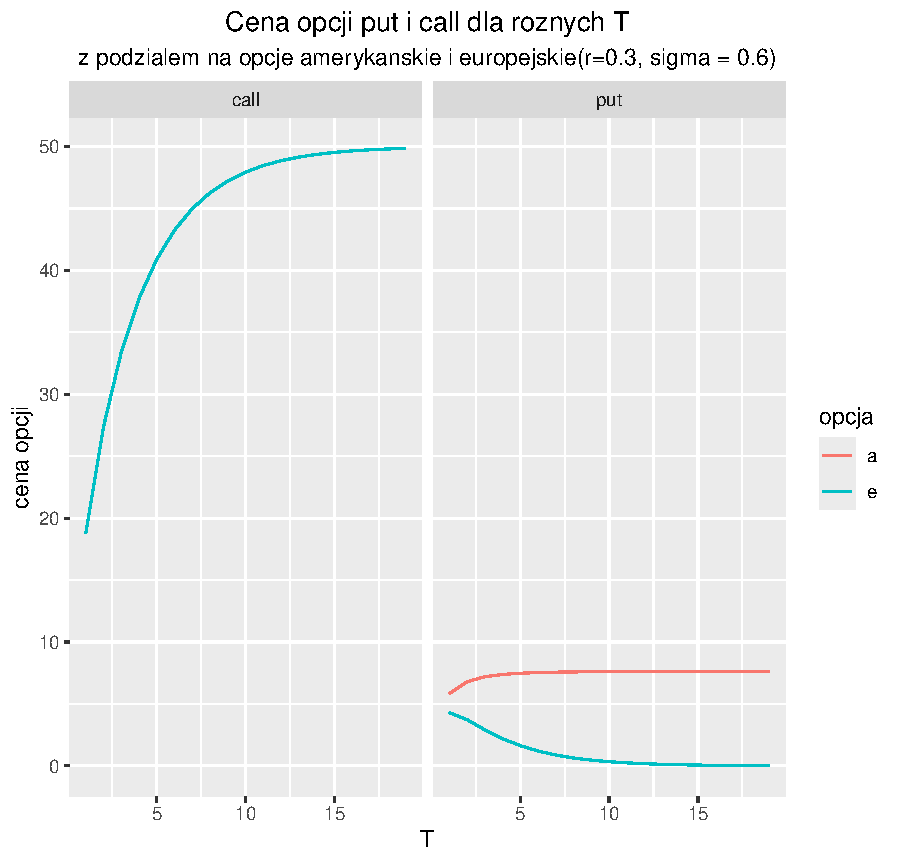
\includegraphics[width=0.4\linewidth]{wykresy/d_r_T_dzikie} \end{center}

\emph{Rysunek 5. Wykres wartości opcji call i put w chwili zero w
zależności od wartości parametrów \(T\), dla większych parametrów \(r\)
i \(\sigma\).}

Widzimy, że w tym przypadku cena opcji europejskiej put również maleje.
Możliwym wytłumaczeniem jest bardzo wysoka stopa wolna od ryzyka: z
opcji put możemy dostać maksymalnie \(K\) (nominalnie, w momencie
\(T\)), więc jeśli czynnik dyskontujący jest duży, a w naszym przypadku
mamy \(e^{-0.3*10}\approx 0.049\), więc maksymalny zysk na chwilę
\(T_0\) jest mały, stąd i mała cena opcji

Przeanalizujmy teraz wpływ parametru \(\Delta t\). Jak widzimy na obu
wykresach, zmienność w uzyskanej wycenie jest bardzo niewielka,
zdecydowanie najmniejsza ze wszystkich rozważanych przypadków. Jest to
również, obok wpływu parametru \(\sigma\), jeden z dwóch przypadków
kiedy wpływ parametru jest taki sam dla obu typów opcji.

Przyjrzyjmy się teraz różnicom w czasach wykonania algorytmu
dokonującego wyceny w zależności od wartości parametru \(\Delta t\).
Poniższy wykres przedstawia uzyskane średnie (obliczone na podstawie 100
powtórzeń) czasy wykonania algorytmu dokonującego wyceny opcji obu typów
i obu rodzajów.

\begin{center}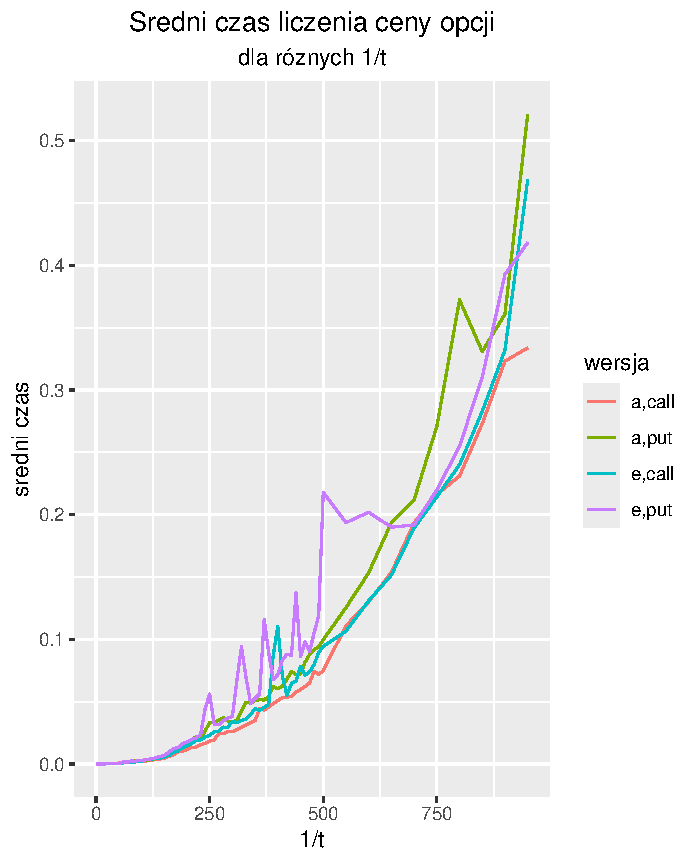
\includegraphics[width=0.4\linewidth]{wykresy/sredni_czas} \end{center}

\emph{Rysunek 6. Wykres średniego (obliczonego na podstawie 1000
powtórzeń) czasu wykonania algorytmu dokonującego wyceny modelem dla
opcji danego typu i rodzaju w zależności od wartości parametru
\(\Delta t\) (oś pozioma przedstawiająca parametr \(\Delta t\) zawiera
jego odwrotności, posortowana rosnąco względem tych odwrotności).}

Pomimo pewnych odchyleń dostrzegamy wyraźny kwadratowy wzrost, wraz ze
wzrostem odwrotności parametru \(\Delta t\) (dla każdego typu i rodzaju
opcji). Oczywiście, uzyskane średnie czasy nawet dla
\(\Delta t = 1/1000\) nie są wysokie, jednak w sytuacji dynamicznej
wyceny nawet kilkuset opcji czas wykonania takiego algorytmu byłby już
znaczący.

\hypertarget{wpux142yw-ruxf3wnoczesnej-zmiany-ruxf3ux17cnych-par-parametruxf3w}{%
\subsection{Wpływ równoczesnej zmiany różnych par
parametrów}\label{wpux142yw-ruxf3wnoczesnej-zmiany-ruxf3ux17cnych-par-parametruxf3w}}

W poprzednich dwóch podrozdziałach analizowaliśmy wpływ zmian
pojedynczych parametrów na uzyskane wyceny opcji na chwilę zero. W tym
podrozdziale przyjrzymy się równoczesnym zmianom różnych par parametrów
w celu dokładniejszej oceny wrażliwości rozważanego modelu. Ze względów
praktycznych (możliwych par jest aż \(15\), co przy dwóch typach opcji
daje łącznie 30 przypadków), analizie poddamy jedynie te przypadki, w
których widoczne są pewne interesujące prawidłowości oraz te, które mogą
reprezentować pewne ważne scenariusze rynkowe (np. różne zmiennośći ceny
aktywa bazowego (parametr \(\sigma\)) wraz ze zmianami stopy
procentowej).

Rozpoczniemy od zbadania wpływu równoczesnych zmian parametrów \(S_0\) i
\(K\). Ponownie, za zakres możliwej zmienności przyjmujemy dla obu
parametrów przedział \([30, 80]\). Pozostałe parametry pozostają
niezmienione, równe wcześniej zaprezentowanym wartościom. Na poniższych
wykresach przedstawiamy uzyskane wyceny opcji call i put na chwilę zero
(podzielone ze względu na rodzaj opcji: a - amerykański, e - europejski)
w formie heatmapy, w zależności od wartości wspomnianych parametrów.

\begin{center}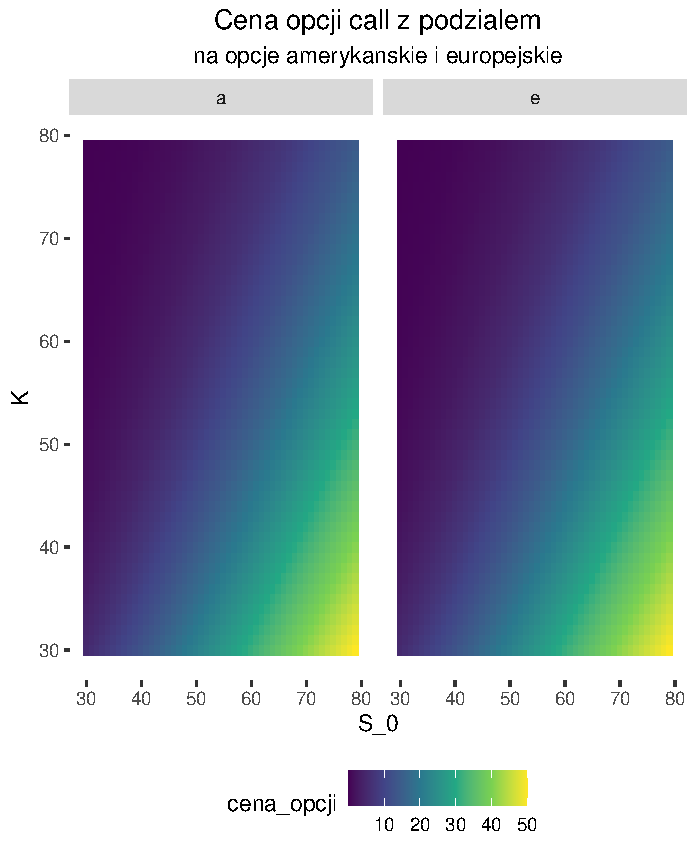
\includegraphics[width=0.45\linewidth]{wykresy/c_r_S0_r_K} 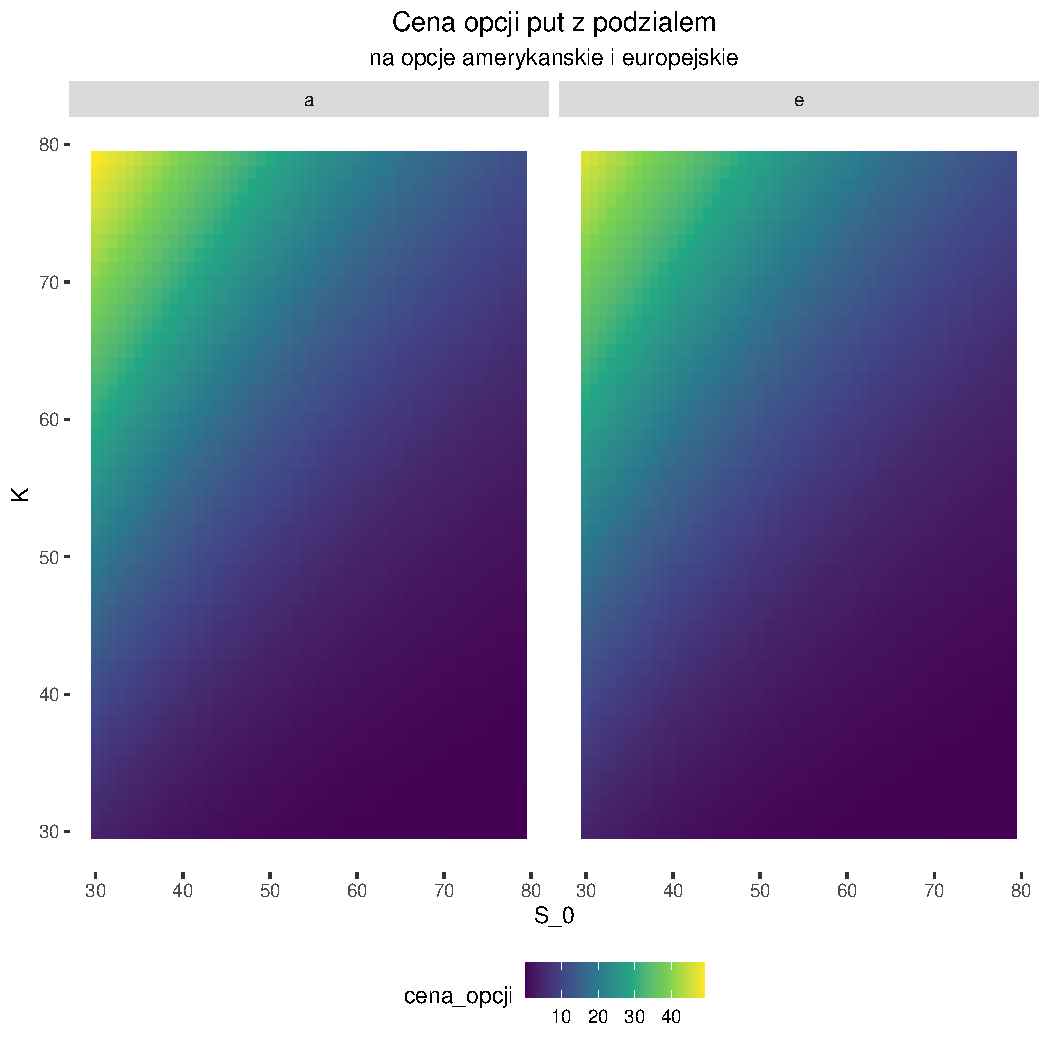
\includegraphics[width=0.45\linewidth]{wykresy/p_r_S0_r_K} \end{center}

\emph{Rysunek 7. Wykres wartości opcji call i put w chwili zero w
zależności od równoczesnej zmiany wartości parametrów \(S_0\) i \(K\).}

Na początku zajmimy się przypadkami opcji call - zarówno dla
amerykańskiej, jak i europejskiej, widzimy ten przebieg -- wartość opcji
rośnie wraz ze wzrostem wartości aktywa bazowego (\(S_0\)) i spadkiem
ceny wykonania (\(K\)). Jest to zgodne z oczekiwaniami, bowiem im wyższa
bieżąca cena aktywa w stosunku do ceny wykonania, tym bardziej opcja
znajduje się „in-the-money'' i tym samym ma wyższą wartość. W przypadku
opcji put, sytuacja wygląda inaczej. Tutaj obserwujemy wzrost wartości
opcji wraz ze wzrostem ceny wykonania i spadkiem wartości aktywa
bazowego, co oznacza (podobnie jak dla opci call), że opcja staje się
bardziej „in-the-money''. Jednak w przeciwieństwie do opcji call, wycena
opcji put różni się dla rodzaju amerykańskiego i europejskiego - nie
jest ona znacząca, ale można dostrzec, że wersja amerykańska przy osiąga
wyższe wartości przy tych samych zmianach obu parametrów.

Przejdźmy teraz do zbadania wpływu równoczesnych zmian parametrów \(r\)
i \(\sigma\). Za zakres możliwej zmienności parametrów przyjmujemy te
same przedziały jak w poprzednim podrozdziale, tj. dla parametru \(r\)
przedział \([-0.03, 0.2]\), a dla parametru przedział \([0.05, 0.3]\).
Pozostałe parametry pozostają niezmienione, równe wcześniej
zaprezentowanym wartościom. Na poniższych wykresach przedstawiamy
uzyskane wyceny opcji call i put na chwilę zero (podzielone ze względu
na rodzaj opcji: a - amerykański, e - europejski) w formie heatmapy, w
zależności od wartości wspomnianych parametrów.

\begin{center}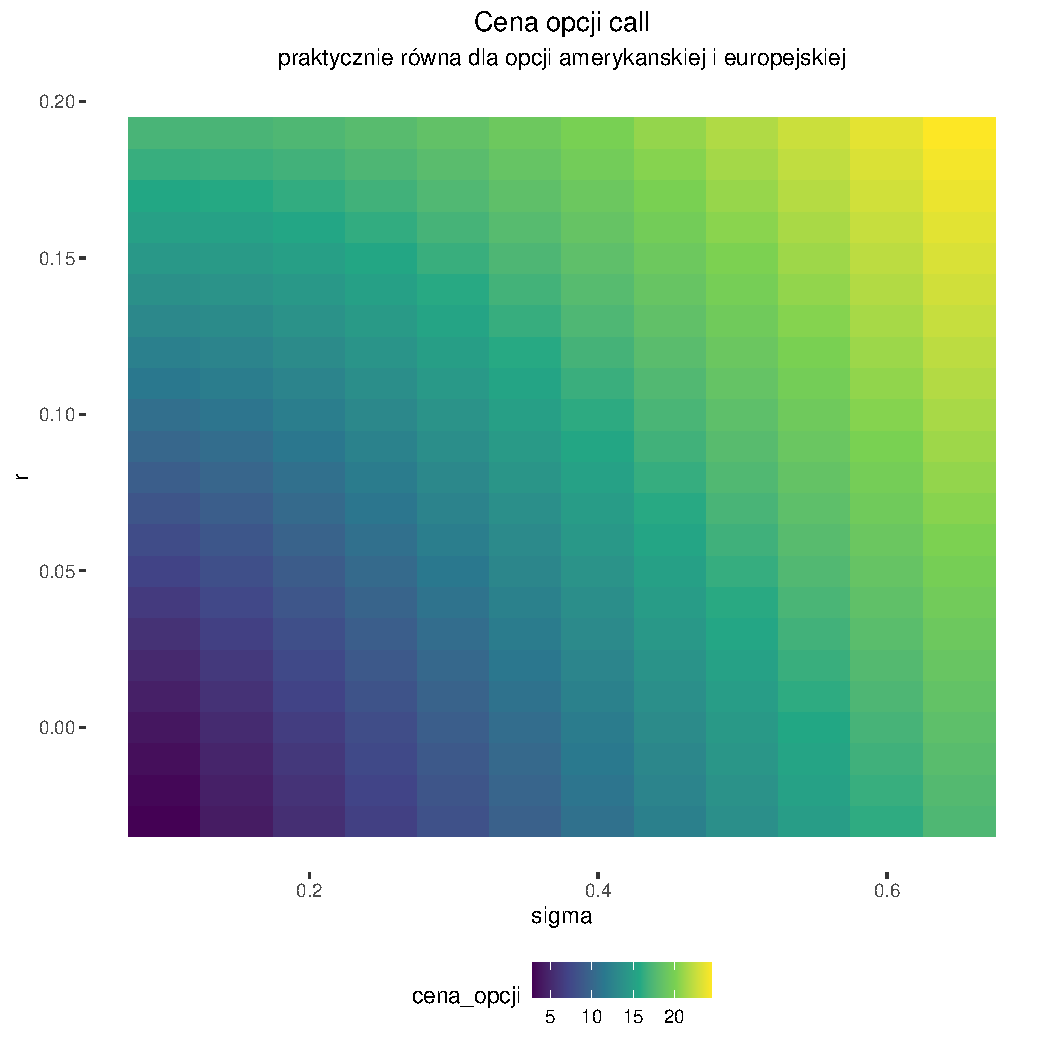
\includegraphics[width=0.45\linewidth]{wykresy/c_r_s_r_r} 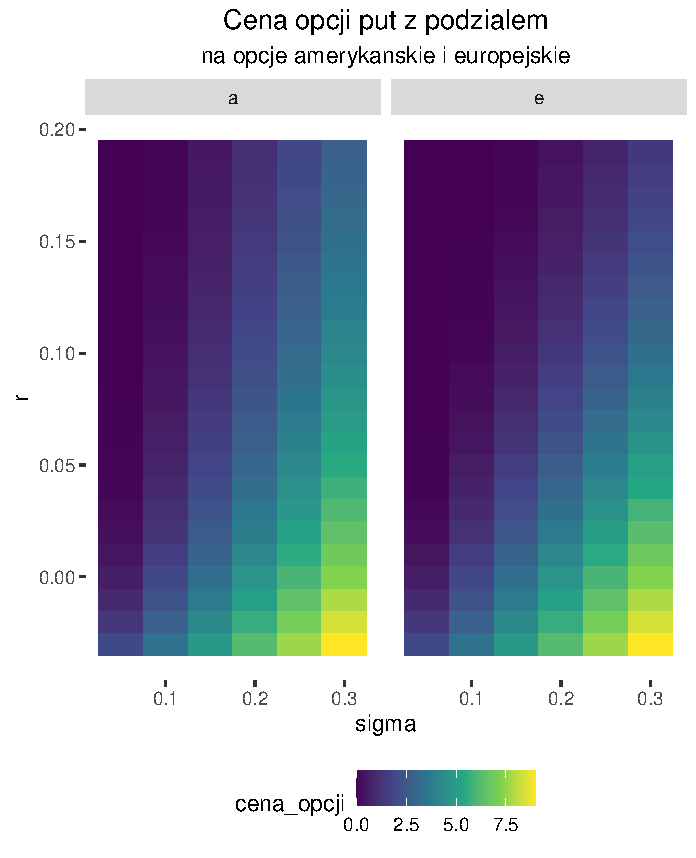
\includegraphics[width=0.45\linewidth]{wykresy/p_r_s_r_r} \end{center}

\emph{Rysunek 8. Wykres wartości opcji call i put w chwili zero w
zależności od równoczesnej zmiany wartości parametrów \(\sigma\) i
\(r\).}

Rozpocznijmy od opcji typu call - dla obu rodzajów opcji (amerykańskich
i europejskich) wartość opcji rośnie wraz ze wzrostem zarówno stopy
procentowej (\(r\)) jak i zmiennością ceny aktywa bazowego (\(\sigma\)).
Wzrost stopy procentowej obniża wartość bieżącą ceny wykonania, co
zwiększa atrakcyjność opcji call. Z kolei wzrost zmienności zwiększa
potencjał skrajnych ruchów ceny aktywa bazowego, co wpływa pozytywnie na
wartość opcji -- dotyczy to w szczególności opcji call, dla których
silne wzrosty ceny aktywa bazowego są korzystne. W przypadku opcji put
również obserwujemy wzrost ceny wraz ze wzrostem zmienności ceny aktywa
bazowego, co jest naturalne -- większa zmienność zwiększa
prawdopodobieństwo, że cena aktywa spadnie znacząco poniżej ceny
wykonania. Jednak w odniesieniu do stopy procentowej, tendencja jest
odwrotna niż dla opcji call - wzrost stopy procentowej powoduje spadek
wartości opcji put. Dzieje się tak, ponieważ wyższe stopy procentowe
zmniejszają bieżącą wartość przyszłych wypłat, które są podstawą wyceny
opcji put. Analogicznie jak w przypadku wpływu parametrów \(S_0\) i
\(K\), warto również zwrócić uwagę na nieco większą wartość opcji put
amerykańskich względem opcji europejskich -- jest to oczywiście
konsekwencja możliwości wcześniejszego wykonania, która w przypadku
opcji put może być korzystna, w szczególności przy niskim poziomie stóp
procentowych i wysokiej zmienności.

\begin{center}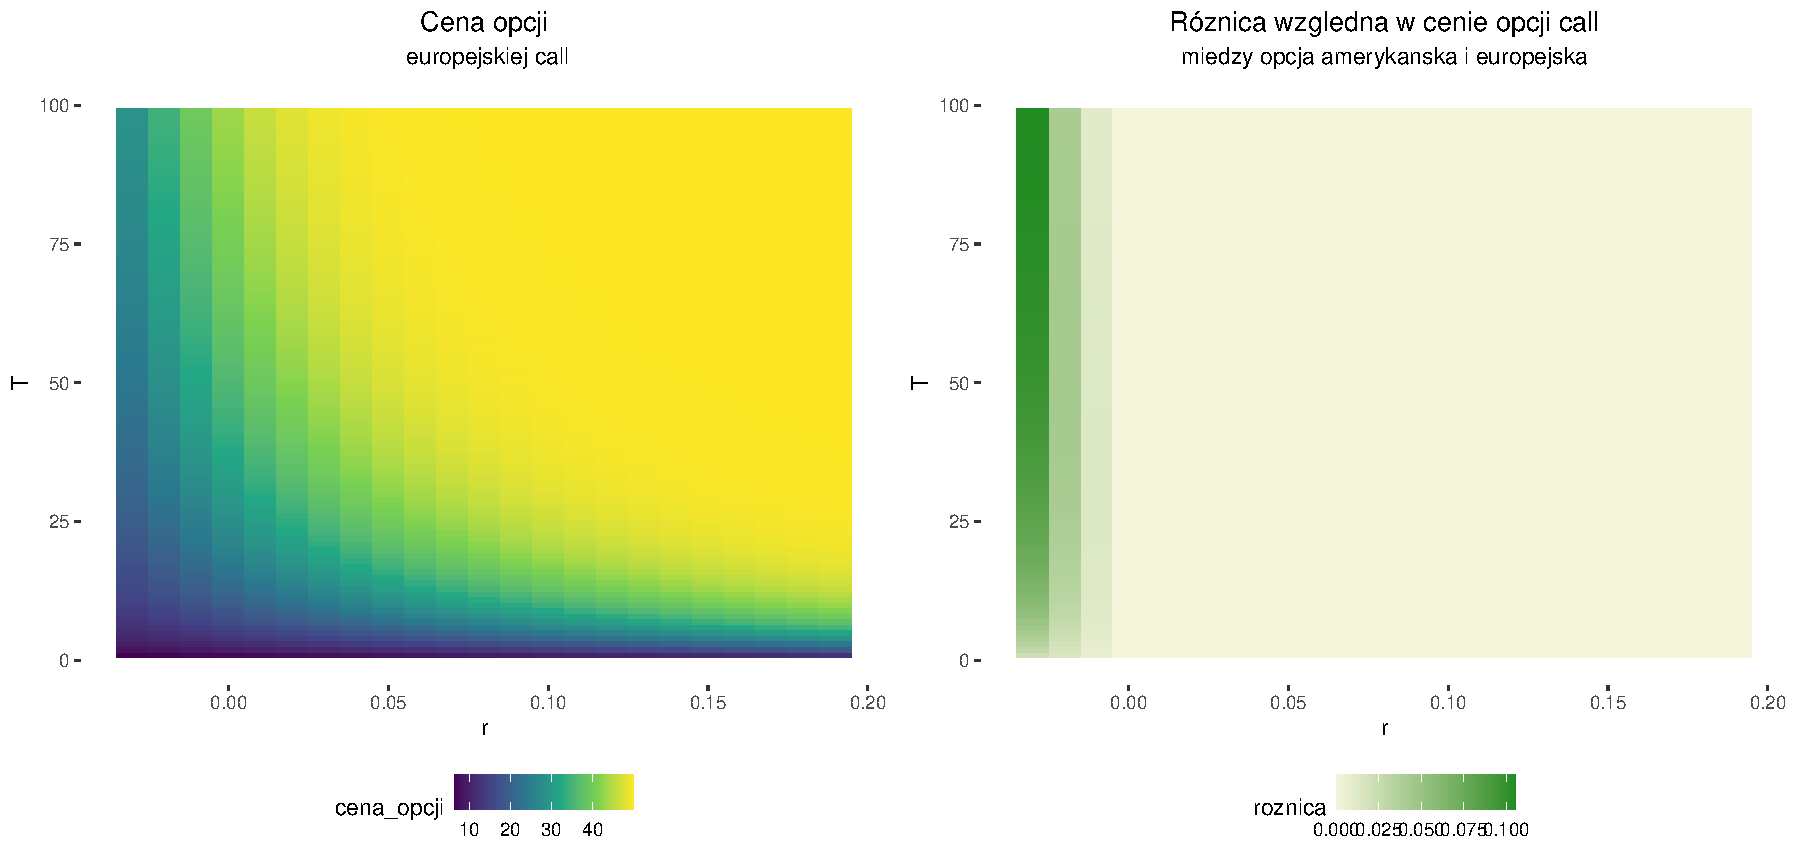
\includegraphics[width=0.45\linewidth]{wykresy/c_r_r_r_T} 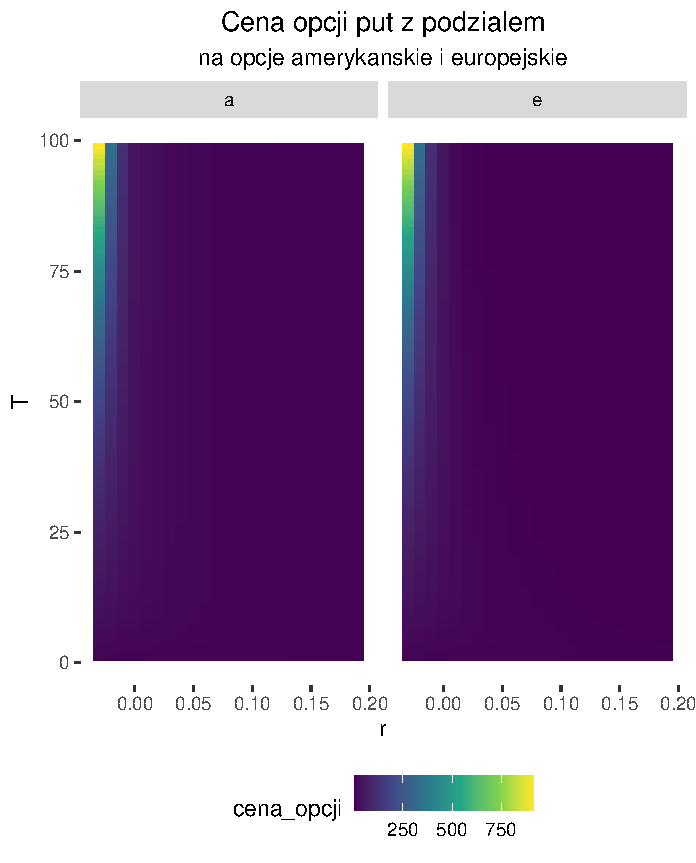
\includegraphics[width=0.45\linewidth]{wykresy/p_r_r_r_T} \end{center}

\emph{Rysunek 9. Wykres wartości opcji call i put w chwili zero w
zależności od równoczesnej zmiany wartości parametrów \(r\) i \(T\)}

Patrząc na poziomice ceny opcji call w zależności od \(T\) oraz \(r\)
możmy zauważyć kształt podobny do hiperboli. Przypominając sobie wzór na
parytet call-put \[C-P-S_0 = -Ke^{-rT},\] Widzimy, że jeśli \(rT\) jest
stały, to również różnica \(C-P\) jest stała. Więc jeśli wartość \(P\)
nie zmienia się znacząco, to również taka zależność będzie zachodzić dla
ceny opcji call

\hypertarget{podsumowanie}{%
\subsection{Podsumowanie}\label{podsumowanie}}

Podsumowanie dokonanych obserwacji rozpoczniemy od tych parametrów, dla
których zmiany w obrębie rozważanych zakresów wywoływały największe
zmiany w uzyskanych wartościach opcji - są to przede wszystkim parametry
\(S_0\), \(K\) oraz \(T\). Zauważmy jednak, że zarówno cena wykonania
jak i czas do wygaśnięcia opcji są dokładnie znane dla każdego
zainteresowanego zawarcia kontraktu opcji, natomiast wartość \(S_0\)
jest nieco inna, bowiem nie jest ona jasno określona. Stosując rozważany
przez nas model wyceny opcji trzeba mieć dużą pewność co do przyjętej
wartości \(S_0\), ponieważ duże odchylenie od jej faktycznej wartości
może doprowadzić do nieprawidłowej wyceny, co w konsekwencji może
skutkować znaczącą stratą pieniężną. Widzimy zatem, że decyzja dotycząca
przyjęcia pewnych wartości parametrów \(K\) i \(T\), pomimo dużej
wpływowości na wycenę, obarczona jest mniejszym ryzykiem niż w przypadku
parametru \(S_0\), ponieważ znacznie ciężej jest tu popełnić błąd -
przyjmuje się po prostu wartości opisane w kontrakcie opcji. Podobny pod
względem możliwości poznania faktycznej wartości jest parametr \(r\),
czyli stopa procentowa od ryzyka; tu również, jak w przypadku parametru
\(S_0\) opierać się trzeba głównie na wartościach krążących na rynku - w
tym przypadku jednak, ewentualny błąd nie jest związany z aż tak dużym
kosztem jak w przypadku parametru \(S_0\). Jeszcze mniejszym wpływem,
czyli tym samym mniejszym potencjalnym kosztem, charakteryzuje się
parametr dotyczący zmienności ceny aktywa bazowego, czyli \(\sigma\).
Tutaj jednak znacznie ciężej o bardzo dokładną estymacje parametru;
każde aktywo bazowe jest inne, co oznacza zupełnie inne możliwości
ewolucji ceny, nie wspominając o nagłych, nieprzewidywalnych
zdarzeniach, które mogą drastycznie ową cenę zmienić - na szczęście, jak
już nadmieniliśmy, wpływ tego parametru nie jest aż tak wielki jak
pozostałych. Na koniec wspomnijmy jeszcze, że parametr \(\Delta t\),
kontrolujący czas mijający w trakcie jednego kroku w drzewie wyceny
(oraz liczbę wierzchołków w owym drzewie) ma bardzo niewielki, wręcz
znikomy wpływ na uzyskaną wartość opcji.

Obserwacje z powyższego akapitu przedstawiamy w uproszczonej formie w
poniższej tabeli.

\begin{longtable}[]{@{}
  >{\raggedright\arraybackslash}p{(\columnwidth - 6\tabcolsep) * \real{0.2500}}
  >{\raggedright\arraybackslash}p{(\columnwidth - 6\tabcolsep) * \real{0.2500}}
  >{\raggedright\arraybackslash}p{(\columnwidth - 6\tabcolsep) * \real{0.2500}}
  >{\raggedright\arraybackslash}p{(\columnwidth - 6\tabcolsep) * \real{0.2500}}@{}}
\toprule()
\begin{minipage}[b]{\linewidth}\raggedright
Parametr
\end{minipage} & \begin{minipage}[b]{\linewidth}\raggedright
Wpływ na wartość opcji call przy wzroście parametru (poziom wpływu)
\end{minipage} & \begin{minipage}[b]{\linewidth}\raggedright
Wpływ na wartość opcji call przy wzroście parametru (poziom wpływu)
\end{minipage} & \begin{minipage}[b]{\linewidth}\raggedright
Ryzyko związane z błędnym wyznaczeniem
\end{minipage} \\
\midrule()
\endhead
\(S_0\) - Początkowa cena aktywa bazowego & dodatni (wysoki) & ujemny
(wysoki) & niskie/średnie \\
\(K\) - Cena wykonania opcji & ujemny (wysoki) & dodatni (wysoki) &
znikome \\
\(\sigma\) - Zmienność ceny aktywa bazowego & dodatni (średni) & dodatni
(średni) & wysokie \\
\(r\) - Stopa procentowa bez ryzyka & dodatni (średni) & ujemny (średni)
& niskie/średnie \\
\(T\) - Czas do wygaśnięcia opcji & dodatni (wysoki) & dodatni (średni)
& znikome \\
\(\Delta t\) - Długość kroku w modelu & znikomy & znikomy & - \\
\bottomrule()
\end{longtable}

\hypertarget{analiza-skux142adu-portfela-zabezpieczajux105cego}{%
\section{Analiza składu portfela
zabezpieczającego}\label{analiza-skux142adu-portfela-zabezpieczajux105cego}}

Na poniższych rysunkach przedstawiono porównanie map ciepła wartości
delty w czasie i pozycjach drzewa binarnego dla opcji typu call oraz
put. Każdy z węzłów drzewa odpowiada konkretnej liczbie wzrostów ceny
instrumentu bazowego oraz momentowi w czasie (na osi X). Kolor w danym
punkcie odzwierciedla wartość delty, czyli liczby akcji potrzebnej w
portfelu zabezpieczającym, aby replikować wartość opcji.

\begin{center}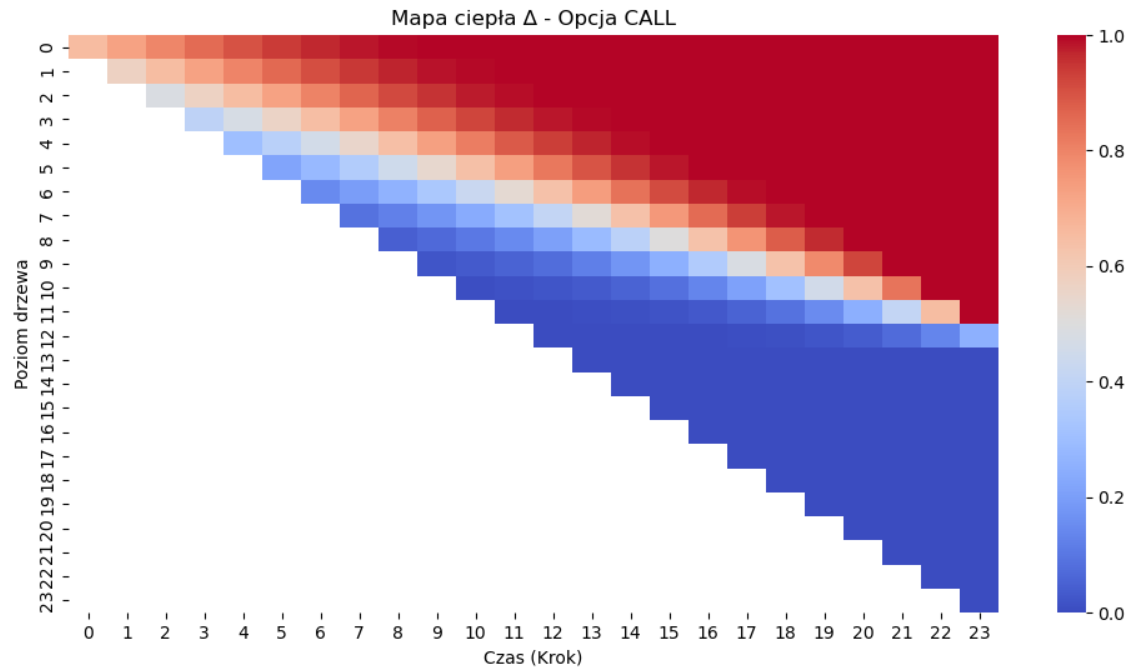
\includegraphics[width=0.75\linewidth]{wykresy/wykres_delta_call} \end{center}

\emph{Rysunek 10. Drzewo wyceny dla opcji call wraz z wartościami delty
w odpowiednich wierzchołkach.}

W przypadku opcji call obserwujemy, że delta rośnie wraz ze wzrostem
ceny instrumentu bazowego i zbliża się do wartości 1 w górnych węzłach
drzewa. Oznacza to, że gdy cena aktywa znacznie przewyższa cenę
wykonania, portfel powinien zawierać prawie jedną akcję, aby skutecznie
odwzorować zachowanie opcji. Z kolei w przypadku opcji put wartość delty
maleje i przyjmuje wartości ujemne, szczególnie w dolnych gałęziach
drzewa, gdzie cena aktywa jest niska. Jednak ze względu na to, że cena
wykonania \(K\) w analizowanym przypadku nie jest znacznie wyższa od
ceny początkowej \(S_{0}\), opcja nie jest głęboko ``in-the-money'',
dlatego delta nie osiąga pełnej wartości \(–1\). Mimo to, zauważalna
jest silna zależność: im niższa cena aktywa bazowego, tym większe
(bardziej ujemne) wartości delty. Porównanie wykresów pozwala dostrzec
symetrię między opcją call a put w kontekście ich wrażliwości na zmianę
ceny instrumentu bazowego, co jest zgodne z teorią finansową. Wartości
delty pozostają w oczekiwanych przedziałach: \([0,1]\) dla call i
\([-1,0]\) dla put, co potwierdza poprawność implementacji modelu.

\begin{center}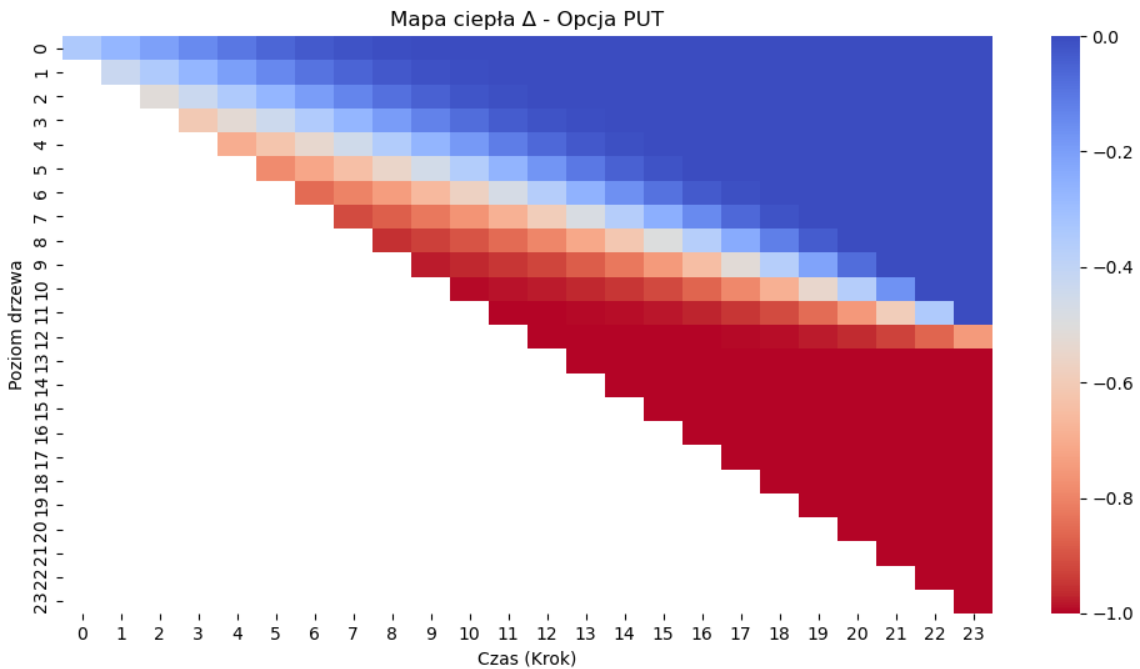
\includegraphics[width=0.75\linewidth]{wykresy/wykres_delta_put} \end{center}

\emph{Rysunek 11. Drzewo wyceny dla opcji put wraz z wartościami delty w
odpowiednich wierzchołkach.}

W przypadku opcji typu put, jak w analizowanym przykładzie, wartości
delty są zazwyczaj ujemne --- oznacza to, że dla zreplikowania opcji
inwestor powinien przyjąć pozycję krótką na akcjach. Można również
zaobserwować, że delta maleje (czyli staje się bardziej ujemna). w
sytuacjach spadków cen instrumentu bazowego. To zgodne z intuicją: im
niższa cena akcji, tym większa wartość opcji put, co wymusza większe
zabezpieczenie przez pozycję przeciwną. Wraz z upływem czasu, czyli w
miarę zbliżania się do terminu wygaśnięcia opcji, wartości delty stają
się bardziej ekstremalne --- to znaczy bardziej zbliżają się do \(-1\)
lub \(0\). Jest to efektem rosnącej wrażliwości wartości opcji na zmiany
ceny aktywa w ostatnich momentach życia opcji. Taka dynamika wymusza
częstsze i bardziej znaczące dostosowania pozycji w portfelu, co
pokazuje rosnące wyzwania związane z praktycznym stosowaniem strategii
delta-hedgingu w końcowych etapach życia opcji.

\newpage

\hypertarget{dodatek-tabela-wykonania-funkcji-i-link-do-repozytorium}{%
\section{Dodatek: Tabela wykonania funkcji i link do
repozytorium}\label{dodatek-tabela-wykonania-funkcji-i-link-do-repozytorium}}

\href{https://github.com/Jankozlowski1234/wdif_projekt}{Link do
repozytorium-github}

W tym dodatkowym podrozdziale zawieramy informacje techniczne dotyczące
implementacji modelu wyceny dwumianowej. Uzyskane wyniki oparte były o
funkcje napisane w języku \emph{Python}.Dane do rysunków od 2 do 7
włącznie były generowane przez funkcje w pliku \emph{main.py} oraz
rysowane w pakiecie \emph{R} w pliku \emph{do\_wykresow.R}. W tabeli
podajemy nazwy funkcji generujących dane, bez nazw plików \emph{.csv}
ponieważ są one długie ale czytelne (np.
\emph{dane\_odwr\_t\_12\_sigma\_0.3\_S\_0\_50\_r\_0.02\_K\_od\_30\_do\_79\_T\_2\_.scv}).
Dodatkowo niepodane parametry dla tych rysunków są ``standerdowe dla
tego zadania'', tj. O\_t = np.array({[}12{]}),Sigmas =
np.array({[}0.3{]}),S\_0 = np.array({[}50{]}),Rs =
np.array({[}0.02{]}),Ks = np.array({[}48{]}),Ts = np.array({[}2{]}).

\begingroup\fontsize{7}{9}\selectfont

\begin{longtable}{ll>{\raggedright\arraybackslash}m{7cm}l}
\toprule
  & nazwa pliku & nazwa funkcji & parametry\\
\midrule
\midrule
\endfirsthead
\multicolumn{4}{@{}l}{\textit{(continued)}}\\
\toprule
  & nazwa pliku & nazwa funkcji & parametry\\
\midrule
\midrule
\endhead

\endfoot
\bottomrule
\endlastfoot
Rysunek 1 & - & - & -\\
\midrule
Rysunek 2 l & - & policz\_dane\_i\_zapisz & S\_0s = np.arange(30, 80, 1)\\
\midrule
Rysunek 2 p & - & policz\_dane\_i\_zapisz & Ks = np.arange(30, 80, 1)\\
\midrule
Rysunek 3 l & - & policz\_dane\_i\_zapisz & Sigmas = np.arange(0.1, 0.66, 0.05)\\
\midrule
Rysunek 3 p & - & policz\_dane\_i\_zapisz & Rs = np.arange(-0.03,0.2, 0.01)\\
\midrule
\addlinespace
Rysunek 4 l & - & policz\_dane\_i\_zapisz & Ts = np.arange(1,100,1)\\
\midrule
Rysunek 4 p & - & policz\_dane\_i\_zapisz & O\_t = np.arange(2, 100, 2)\\
\midrule
Rysunek 5 & - & policz\_dane\_i\_zapisz & \makecell[c]{Ts = np.arange(1,20,1),Rs = np.array([0.3]), \\ Sigmas = np.array([0.6])}\\
\midrule
Rysunek 6 & - & zbadaj\_ile\_liczy\_srednio\_wszystkie\_mozliwosci & \makecell[r]{N = 1000,\\ O\_t = (np.arange(1,100,2),\\ np.arange(100,500,10),np.arange(500,1000,50))}\\
\midrule
Rysunek 7 & - & policz\_dane\_i\_zapisz & \makecell[l]{S\_0s = np.arange(30, 80, 1), \\Ks = np.arange(30, 80, 1)}\\
\midrule
\addlinespace
Rysunek 8 & - & policz\_dane\_i\_zapisz & \makecell[c]{Sigmas = np.arange(0.1, 0.66, 0.05),\\ Rs = np.arange(-0.03,0.2, 0.01)}\\
\midrule
Rysunek 9 & - & policz\_dane\_i\_zapisz & \makecell[r]{Ts = np.arange(1,100,1),\\                       \\ Rs = np.arange(-0.03,0.2, 0.01)}\\
\midrule
Rysunek 10 & - & plot\_delta\_heatmap & opcyja = 'CALL'\\
\midrule
Rysunek 11 & - & plot\_delta\_heatmap & opcyja = 'PUT'\\
\midrule*
\end{longtable}
\endgroup{}

\end{document}
